\documentclass[aspectratio=1610,onlymath]{beamer}
% \documentclass[aspectratio=1610,onlymath,handout]{beamer}

\input{macros-lecture}
% Common notation

\usepackage{amsmath,amssymb,amsfonts}
\usepackage{xspace}

\newcommand{\lectureurl}{https://iccl.inf.tu-dresden.de/web/FS2023}

\DeclareMathAlphabet{\mathsc}{OT1}{cmr}{m}{sc} % Let's have \mathsc since the slide style has no working \textsc

% Dual of "phantom": make a text that is visible but intangible
\newcommand{\ghost}[1]{\raisebox{0pt}[0pt][0pt]{\makebox[0pt][l]{#1}}}

\newcommand{\tuple}[1]{\langle{#1}\rangle}
\newcommand{\defeq}{\mathrel{:=}}

%%% Annotation %%%

\usepackage{color}
\newcommand{\todo}[1]{{\tiny\color{red}\textbf{TODO: #1}}}



%%% Old macros below; move when needed

\newcommand{\blank}{\text{\textvisiblespace}} % empty tape cell for TM

% table syntax
\newcommand{\dom}{\textbf{dom}}
\newcommand{\adom}{\textbf{adom}}
\newcommand{\dbconst}[1]{\texttt{"#1"}}
\newcommand{\pred}[1]{\textsf{#1}}
\newcommand{\foquery}[2]{#2[#1]}
\newcommand{\ground}[1]{\textsf{ground}(#1)}
% \newcommand{\foquery}[2]{\{#1\mid #2\}} %% Notation as used in Alice Book
% \newcommand{\foquery}[2]{\tuple{#1\mid #2}}

\newcommand{\quantor}{\mathord{\reflectbox{$\text{\sf{Q}}$}}} % the generic quantor

% logic syntax
\newcommand{\Inter}{\mathcal{I}} %used to denote an interpretation
\newcommand{\Jnter}{\mathcal{J}} %used to denote another interpretation
\newcommand{\Knter}{\mathcal{K}} %used to denote yet another interpretation
\newcommand{\Zuweisung}{\mathcal{Z}} %used to denote a variable assignment

% query languages
\newcommand{\qlang}[1]{{\sf #1}} % Font for query languages
\newcommand{\qmaps}[1]{\textbf{QM}({\sf #1})} % Set of query mappings for a query language

%%% Complexities %%%

\hyphenation{Exp-Time} % prevent "Ex-PTime" (see, e.g. Tobies'01, Glimm'07 ;-)
\hyphenation{NExp-Time} % better that than something else

% \newcommand{\complclass}[1]{{\sc #1}\xspace} % font for complexity classes
\newcommand{\complclass}[1]{\ensuremath{\mathsc{#1}}\xspace} % font for complexity classes

\newcommand{\ACzero}{\complclass{AC$_0$}}
\newcommand{\LogSpace}{\complclass{L}}
\newcommand{\NLogSpace}{\complclass{NL}}
\newcommand{\PTime}{\complclass{P}}
\newcommand{\NP}{\complclass{NP}}
\newcommand{\coNP}{\complclass{coNP}}
\newcommand{\PH}{\complclass{PH}}
\newcommand{\PSpace}{\complclass{PSpace}}
\newcommand{\NPSpace}{\complclass{NPSpace}}
\newcommand{\ExpTime}{\complclass{ExpTime}}
\newcommand{\NExpTime}{\complclass{NExpTime}}
\newcommand{\ExpSpace}{\complclass{ExpSpace}}
\newcommand{\TwoExpTime}{\complclass{2ExpTime}}
\newcommand{\NTwoExpTime}{\complclass{N2ExpTime}}
\newcommand{\ThreeExpTime}{\complclass{3ExpTime}}
\newcommand{\kExpTime}[1]{\complclass{#1ExpTime}}
\newcommand{\kExpSpace}[1]{\complclass{#1ExpSpace}}


\defineTitle{10}{Grenzen regulärer Sprachen / Probleme~für~Automaten}{26. November 2020}

\begin{document}

\maketitle

\sectionSlideNoHandout{Rückblick}

\begin{frame}\frametitle{Minimale Automaten}

Für jede reguläre Sprache $\Slang{L}$
\begin{enumerate}[\ldots]
\item gibt es einen minimalen (totalen) DFA 
\item der eindeutig ist bis auf Umbenennung von Zuständen
\item den man durch Reduktion jedes beliebigen DFA für $\Slang{L}$ erhalten kann
\item oder auch als Myhill-Nerode-Minimalautomat
\end{enumerate}
\bigskip

Allerdings ist der minimale DFA unter Umständen viel größer als ein minimaler NFA
(dafür ist letzterer schwerer zu finden und nicht eindeutig)

\end{frame}


\sectionSlide{Nichtreguläre Sprachen}

\begin{frame}\frametitle{Nichtreguläre Sprachen}

Sind alle Sprachen regulär?\\
\redalert{Sicher nicht} (dazu gibt es zu viele Sprachen)
\bigskip

Sind alle Typ-0-Sprachen regulär?\\
\redalert{Nein,} auch das gilt nicht
\bigskip

\alert{Wie aber zeigt man das?}
\begin{itemize}
\item Behauptung "`Sprache $\Slang{L}$ ist regulär!"' $\leadsto$ es genügt, \alert{einen} Automaten, regulären Ausdruck oder eine Typ-3-Grammatik für $\Slang{L}$ anzugeben
\item Behauptung "`Sprache $\Slang{L}$ ist nicht regulär!"' $\leadsto$ man müsste zeigen, dass es \alert{keinen} Automaten, \alert{keinen} regulären Ausdruck bzw. \alert{keine} Typ-3-Grammatik für $\Slang{L}$ gibt
\end{itemize}

\end{frame}

\begin{frame}\frametitle{Nichtregularität mit Myhill \& Nerode}

Myhill \& Nerode liefern uns ein besseres Kriterium:

\theobox{\emph{Satz (Myhill \& Nerode):} Eine Sprache $\Slang{L}$ ist genau dann regulär, wenn $\simeq_{\Slang{L}}$ endlich viele Äquivalenzklassen hat.}\medskip

Daraus folgt:

\theobox{\emph{Satz:} Wenn $\simeq_{\Slang{L}}$ unendlich viele Äquivalenzklassen hat, dann ist $\Slang{L}$ nicht regulär.}%
\medskip\pause

\examplebox{\emph{Beispiel:} Wir haben gesehen, dass die Sprache $\{\Sterm{a}^n\Sterm{b}^n\mid n\geq 0\}$
unendlich viele Äquivalenzklassen erzeugt. Diese Sprache ist demnach nicht regulär.}

\end{frame}

\begin{frame}\frametitle{$\Sterm{a}^n\Sterm{b}^n$}

Die Sprache $\Sterm{a}^n\Sterm{b}^n$ gilt als Musterbeispiel nichtregulärer Sprachen
\bigskip

\anybox{purple}{Intuition: "`Reguläre Sprachen können nicht zählen."'}%
\bigskip

Ein Automat, der diese Sprache erkennen wollte, müsste die genaue Zahl der schon gelesenen $\Sterm{a}$s speichern
\medskip

$\leadsto$ beliebig viel Speicher nötig
\bigskip

Viele Sprachdefinitionen mit Bezug zu konkreten Zahlen verhalten sich ähnlich

\end{frame}

\begin{frame}[t]\frametitle{Nichtregularität mit Abschlusseigenschaften}

Wir haben bereits gezeigt:

\theobox{\emph{Satz:} Wenn $\Slang{L}_1$ und $\Slang{L}_2$ regulär sind, dann auch $\Slang{L}_1\cap \Slang{L}_2$,
$\Slang{L}_1\cup \Slang{L}_2$, $\Slang{L}_1^*$ und $\overline{\Slang{L}}_1$.}\medskip

Auch hier liefert die Umkehrung gute Kriterien, z.B.
\theobox{\emph{Satz:} Wenn $\Slang{L}_1$ regulär und $\Slang{L}_1\cap \Slang{L}_2$ nicht regulär ist, dann ist
$\Slang{L}_2$ ebenfalls nicht regulär.}\medskip\pause

\examplebox{\emph{Beispiel:} Wir betrachten über dem Alphabet $\{\Sterm{a},\Sterm{b}\}$ die Sprache\\ $\Slang{L}=\{w\mid w\text{ enthält ebenso viele $\Sterm{a}$ wie $\Sterm{b}$}\}$.
\medskip

\only<3->{Dann gilt $\Slang{L}\cap \{\Sterm{a}\}^*\{\Sterm{b}\}^* = \{\Sterm{a}^n\Sterm{b}^n\mid n\geq 0\}$.
\medskip

Weil $\{\Sterm{a}\}^*\{\Sterm{b}\}^*$ regulär ist und $\{\Sterm{a}^n\Sterm{b}^n\mid n\geq 0\}$ nicht, kann
$\Slang{L}$ ebenfalls nicht regulär sein.}
}

\end{frame}

% \begin{frame}[t]\frametitle{Nichtregularität mit Abschlusseigenschaften (2)}
% 
% Noch ein Beispiel: Komplement der gerade gezeigten Sprache
% 
% \end{frame}

\newcommand{\colstackrel}[3]{\,{\stackrel{\textcolor{#3}{#1}}{\textcolor{#3}{#2}}}\,}
\newcommand{\gstackrel}[2]{\colstackrel{#1}{#2}{darkgreen}}
\newcommand{\bstackrel}[2]{\colstackrel{#1}{#2}{darkblue}}
\newcommand{\rstackrel}[2]{\colstackrel{#1}{#2}{darkred}}

\begin{frame}\frametitle{Nichtregularität durch Pumpen}

Ein weiteres klassisches Kriterium für Nichtregularität ist, dass die Wörter regulärer Sprachen
beliebig "`aufgepumpt"' werden können.
\bigskip

\emph{Idee:}
\begin{itemize}
\item Jeder DFA hat nur endlich viele Zustände $n$
\item Aber manche reguläre Sprachen enthalten beliebig lange Wörter
\end{itemize}
\narrowcentering{\alert{Wie kann ein DFA Wörter mit mehr als $n$ Zeichen akzeptieren?}}\pause
% \bigskip
% 
\begin{itemize}
\item Dann muss der DFA beim Einlesen einen Zustand mehr als einmal besuchen
\item Dafür muss es in den Zustandsübergangen eine Schleife geben
\item Diese Schleife kann man aber auch mehr als einmal durchlaufen
% 
% % \item Was passiert wenn der DFA ein Wort mit $|w|>n$ akzeptiert?
% % \item In diesem Fall muss er mindestens einen Zustand mehr als einmal annehmen
% \item Akzeptiert ein DFA ein Wort mit $\geq n$ Zeichen, dann muss er also einen Zustand mehr als einmal besuchen
% \item 
% \item Wenn der DFA die Schleife einmal durchlaufen kann, dann kann er sie auch beliebig oft durchlaufen
% \item daher muss der Automat beliebig viele 
\end{itemize}\pause

\begin{center}
\alert{Jedes akzeptierte Wort mit $\geq n$ Zeichen hat einen Teil, den man beliebig oft wiederholen -- "`aufpumpen"' -- kann}
\end{center}

\end{frame}

\begin{frame}\frametitle{Das Pumping-Lemma}

\theobox{\emph{Satz (Pumping-Lemma):}
Für jede reguläre Sprache $\Slang{L}$\\
gibt es eine Zahl $n\geq 0$, so dass gilt:\\
~~für jedes Wort $z\in\Slang{L}$ mit $|z|\geq n$\\
~~gibt es eine Zerlegung $z=uvw$ mit $|v|\geq 1$ und $|uv|\leq n$, so dass:\\
~~~~für jede Zahl $k\geq 0$ gilt: $u v^k w\in\Slang{L}$
}

\pause
\emph{Beweis:} Sei $\Smach{M}$ ein DFA für $\Slang{L}$ mit $|Q|$ Zuständen. \pause
Wir wählen $n=|Q|+1$.\\\pause Ein akzeptierender Lauf für ein beliebiges Wort $z$ mit $|z|=\ell\geq n$
muss in den ersten $n$ Schritten einen Zustand $p$ zweimal besuchen (sagen wir: nach $i$ und $j$ Schritten),
hat also die Form:
% Es gibt also Zahlen mit $0\leq i<j\leq n$ für die der Lauf folgende Form hat:
% Der Lauf hat also folgende Form:
%
\[ q_0 \gstackrel{z_1}{\to}q_1\gstackrel{z_2}{\to}\!\ldots\!\gstackrel{z_{i-1}}{\to}q_{i-1}\gstackrel{z_i}{\to} p\bstackrel{z_{i+1}}{\to} q_{i+1}\bstackrel{z_{i+2}}{\to}\!\ldots\!\bstackrel{z_{j-1}}{\to}q_{j-1}\bstackrel{z_j}{\to} p \rstackrel{z_{j+1}}{\to}q_{j+1}\rstackrel{z_{j+2}}{\to}\!\ldots\!\rstackrel{z_\ell}{\to}q_\ell\]
%
\pause Die gesuchte Zerlegung ist $u\,{=}\,\textcolor{darkgreen}{z_1\cdots z_i}$, $v\,{=}\,\textcolor{darkblue}{z_{i+1}\cdots z_{j}}$, $w\,{=}\,\textcolor{darkred}{z_{j+1}\cdots z_\ell}$.\\ \pause
Der Lauf $(q_0\ldots q_{i-1} p) (q_{i+1}\ldots q_{j-1}p)^k (q_{j+1}\ldots q_\ell)$ akzeptiert $uv^k w$.
% 
% Akzeptierende Läufe für $uv^k w$.
% 
% 
% Es gibt also einen
% Zyklus $q\stackrel{v}{\to}q$. Die Behauptung folgt, da man diesen Zyklus beliebig oft durchlaufen kann.
\qed

\end{frame}

\begin{frame}\frametitle{Beispiel}

\examplebox{%
\emph{Beispiel:} Die Sprache von $\Sterm{b}^*(\Sterm{a}\Sterm{b}^*\Sterm{a}\Sterm{b}^*)^*$ (Wörter mit gerader Anzahl $\Sterm{a}s$).
Der Parameter $n$ aus dem Pumping-Lemma kann $2$ sein:
\begin{itemize}
\item Wenn $z$ die Form $\Sterm{b}y$ hat, wähle $u=\epsilon$, $v=\Sterm{b}$ und $w=y$
\item Wenn $z$ die Form $\Sterm{ab}y$ hat, wähle $u=\Sterm{a}$, $v=\Sterm{b}$ und $w=y$
\item Wenn $z$ die Form $\Sterm{aa}y$ hat, wähle $u=\epsilon$, $v=\Sterm{aa}$ und $w=y$
\end{itemize}
}\medskip\pause

\examplebox{\emph{Beispiel:} Für endliche Sprachen ist die Eigenschaft trivial. Man wählt $n$ einfach so groß, dass
es keine Wörter $z$ mit $|z|\geq n$ gibt, für welche weitere Eigenschaften gefordert werden.}

\end{frame}

\begin{frame}[t]\frametitle{Pumpen für Nichtregularität}

Die Pump-Eigenschaft ist für Regularität \alert{notwendig}, aber \alert{nicht hinreichend}: man kann auch manche nichtreguläre Sprachen pumpen.
\medskip

Daher eignet sich das Pumping-Lemma eher zum Beweis der Nichtregularität
\medskip\pause

\examplebox{\emph{Beispiel:} Sei $\Slang{L}=\{\Sterm{a}^k\mid k\text{ ist Primzahl}\}$.
\only<3->{\medskip

Angenommen es gäbe einen Wert $n$ für den diese Sprache aufgepumpt werden kann.
Es gibt eine Primzahl $\ell>n+2$.
Laut Pump-Eigenschaft finden wir eine Zerlegung von $\Sterm{a}^\ell=uvw$
für die insbesondere gilt $uv^{|uw|}w\in\Slang{L}$.
Aber $uv^{|uw|}w=\Sterm{a}^{(k+1)|uw|}\notin\Slang{L}$. Widerspruch.\medskip

$\Slang{L}$ ist daher nicht regulär.}
}

\end{frame}


\begin{frame}\frametitle{Ist das Pumping-Lemma sinnvoll?}

% Diskussion:
\begin{itemize}
\item \emph{Kontra:} Myhill-Nerode liefert ein notwendiges \redalert{und} hinreichendes Kriterium für Regularität\\
$\leadsto$ immer anwendbar, um (Nicht)Regularität zu zeigen
\item \emph{Pro:} Pumping funktioniert in den allermeisten praktischen Fällen auch\\
(notfalls kann man Abschlusseigenschaften zu Hilfe nehmen)
\item \emph{Pro:} Manchmal ist der Beweis mit Pumping einfacher
\item \emph{Kontra:} Das formale Pumping-Lemma ist relativ kompliziert
\item \emph{Pro:} Die Pumping-Idee ist intuitiv und wir werden sie später noch einmal bei kontextfreien Sprachen nutzen
\end{itemize}

\end{frame}

% \begin{frame}\frametitle{Pumpen zur Größenabschätzung}
% \end{frame}

\sectionSlide{Algorithmen für Automaten}

% \begin{frame}\frametitle{Berechnungen auf endlichen Automaten}
% 
% \begin{tabular}{rl}
%  & \\
% \end{tabular}
% 
% \end{frame}

\begin{frame}[t]\frametitle{Wichtige Probleme für Sprachen}

\defbox{
Das \redalert{Wortproblem} für eine Sprache $\Slang{L}$ über Alphabet $\Sigma$ besteht darin, die folgende Funktion zu berechnen:\\[1ex]
\emph{Eingabe:} ein Wort $w\in\Sigma^*$\\
\emph{Ausgabe:} "`ja"' wenn $w\in\Slang{L}$ und "`nein"' wenn $w\notin\Slang{L}$
}

Ziel bei der Lösung des Wortproblems:
\begin{itemize}
\item Finde einen Algorithmus, der diese Funktion berechnet
\item Die Sprache $\Slang{L}$ ist \alert{nicht} Teil der Eingabe, sondern fester Bestandteil des Algorithmus
\item Es ist daher unerheblich, wie wir Sprachen darstellen (Grammatik, Automat, \ldots)
\end{itemize}

\end{frame}

\begin{frame}[t]\frametitle{Wichtige Probleme für Automaten}

% Andererseits kann man auch Probleme für FAs finden:

\defbox{
Das \redalert{Wortproblem} für FAs über Alphabet $\Sigma$ besteht darin, die folgende Funktion zu berechnen:\\[1ex]
\emph{Eingabe:} ein FA $\Smach{M}$ und ein Wort $w\in\Sigma^*$\\
\emph{Ausgabe:} "`ja"' wenn $w\in\Slang{L}(\Smach{M})$ und "`nein"' wenn $w\notin\Slang{L}(\Smach{M})$
}

\begin{itemize}
\item Hier ist die Sprache (gegeben als FA) Teil der Eingabe
\item Die Repräsentation (DFA oder NFA?) spielt unter Umständen eine wichtige Rolle 
\end{itemize}\pause

\defbox{
Das \redalert{Leerheitsproblem} für FAs über Alphabet $\Sigma$ besteht darin, die folgende Funktion zu berechnen:\\[1ex]
\emph{Eingabe:} ein FA $\Smach{M}$ über Alphabet $\Sigma$\\
\emph{Ausgabe:} "`ja"' wenn $\Slang{L}(\Smach{M})=\emptyset$ und "`nein"' wenn $\Slang{L}(\Smach{M})\neq\emptyset$
}

\end{frame}

\begin{frame}\frametitle{Wichtige Probleme für Automaten (2)}

% Wichtig ist auch der Vergleich zweier durch Automaten gegebener Sprachen:

\defbox{
Das \redalert{Inklusionsproblem} für FAs über Alphabet $\Sigma$ besteht darin, die folgende Funktion zu berechnen:\\[1ex]
\emph{Eingabe:} zwei FAs $\Smach{M}_1$ und $\Smach{M}_2$ über Alphabet $\Sigma$\\
\emph{Ausgabe:} "`ja"' wenn $\Slang{L}(\Smach{M}_1)\subseteq\Slang{L}(\Smach{M}_2)$; andernfalls "`nein"'
}

\defbox{
Das \redalert{Äquivalenzproblem} für FAs über Alphabet $\Sigma$ besteht darin, die folgende Funktion zu berechnen:\\[1ex]
\emph{Eingabe:} zwei FAs $\Smach{M}_1$ und $\Smach{M}_2$ über Alphabet $\Sigma$\\
\emph{Ausgabe:} "`ja"' wenn $\Slang{L}(\Smach{M}_1)=\Slang{L}(\Smach{M}_2)$; andernfalls "`nein"'
}\pause

Manche Probleme kann man mittels anderer ausdrücken:
\begin{itemize}
\item $\Slang{L}(\Smach{M}_1)=\Slang{L}(\Smach{M}_2)$ gdw. $\Slang{L}(\Smach{M}_1)\subseteq\Slang{L}(\Smach{M}_2)$ und $\Slang{L}(\Smach{M}_2)\subseteq\Slang{L}(\Smach{M}_1)$
\item $\Slang{L}(\Smach{M})=\emptyset$ gdw. $\Slang{L}(\Smach{M})\subseteq\Slang{L}(\Smach{M}_\emptyset)$, wobei 
$\Smach{M}_\emptyset$ ein FA ist, der keine Wörter akzeptiert
\end{itemize}
Wir werden noch mehr solche \alert{Reduktionen} sehen

\end{frame}

\begin{frame}\frametitle{Das Leerheitsproblem für DFA und NFA}

\defbox{
Das \redalert{Leerheitsproblem} für FAs über Alphabet $\Sigma$ besteht darin, die folgende Funktion zu berechnen:\\[1ex]
\emph{Eingabe:} ein FA $\Smach{M}$ über Alphabet $\Sigma$\\
\emph{Ausgabe:} "`ja"' wenn $\Slang{L}(\Smach{M})=\emptyset$ und "`nein"' wenn $\Slang{L}(\Smach{M})\neq\emptyset$
}

\emph{Anwendungsbeispiel:}
Konsistenzprüfung einer Systemspezifikation
\begin{itemize}
\item In der formalen Verifikation kann (erwünschtes) Systemverhalten mit Automaten dargestellt werden
\item Wörter entsprechen z.B. erlaubten Programmdurchläufen
\item Leerheitstest: prüfe, ob die Spezifikation überhaupt erfüllt werden kann
\end{itemize}

\end{frame}

\begin{frame}\frametitle{Komplexität des Leerheitsproblems}

Das Leerheitsproblem ist leicht zu lösen:

\theobox{\emph{Satz:} Die Leerheit eines NFA (oder auch DFA) kann in polynomieller Zeit entschieden werden.}

\pause
\emph{Beweis:} Leerheit = "`Es gibt keinen von einem Startzustand aus erreichbaren Endzustand"'
\bigskip

Erreichbarkeit von Endzuständen kann mithilfe von Graphalgorithmen zur Erreichbarkeitsprüfung (Breadth-First-Search, Depth-First-Search, \ldots) getestet werden. Einfache Algorithmen laufen in $O(|Q|\times |\delta|)$, wobei $|Q|$ die Zahl der Zustände und $|\delta|$ die Gesamtzahl der Kanten im Graph des Automaten ist.\qed

\end{frame}

\begin{frame}\frametitle{Das Inklusionsproblem für DFA und NFA}

\defbox{
Das \redalert{Inklusionsproblem} für FAs über Alphabet $\Sigma$ besteht darin, die folgende Funktion zu berechnen:\\[1ex]
\emph{Eingabe:} zwei FAs $\Smach{M}_1$ und $\Smach{M}_2$ über Alphabet $\Sigma$\\
\emph{Ausgabe:} "`ja"' wenn $\Slang{L}(\Smach{M}_1)\subseteq\Slang{L}(\Smach{M}_2)$; andernfalls "`nein"'
}

\emph{Anwendungsbeispiel:}
Verifikation einer Systemspezifikation
\begin{itemize}
\item Spezifiziere erwünschtes Systemverhalten als Automat $\Smach{M}_{\text{spec}}$
\item Abstrahiere tatsächliches Systemverhalten durch Automat $\Smach{M}_{\text{sys}}$
\item Inklusionstest $\Slang{L}(\Smach{M}_{\text{sys}})\subseteq\Slang{L}(\Smach{M}_{\text{spec}})$: Prüfe, ob System Spezifikation erfüllt
\end{itemize}

\end{frame}

\begin{frame}\frametitle{Lösen des Inklusionsproblems}

Wie kann man $\Slang{L}(\Smach{M}_1)\subseteq\Slang{L}(\Smach{M}_2)$ testen?\pause
\bigskip

\emph{Reduktion auf Leerheitsproblem:}\medskip

\begin{tabular}{r@{~~~ gdw ~~~}l}
$\Slang{L}(\Smach{M}_1)\subseteq\Slang{L}(\Smach{M}_2)$
	& für jedes $w\in \Slang{L}(\Smach{M}_1)$ gilt $w\in \Slang{L}(\Smach{M}_2)$\\\pause
	& es gibt kein $w\in\Slang{L}(\Smach{M}_1)$ mit $w\notin\Slang{L}(\Smach{M}_2)$ \\\pause
	& es gibt kein $w\in\Slang{L}(\Smach{M}_1)\cap (\Sigma^*\setminus\Slang{L}(\Smach{M}_2))$ \\\pause
	& $\Slang{L}(\Smach{M}_1)\cap (\Sigma^*\setminus\Slang{L}(\Smach{M}_2))=\emptyset$ \\\pause
	& $\Slang{L}(\Smach{M}_1)\cap\overline{\Slang{L}(\Smach{M}_2)}= \emptyset$ \\\pause
	& $\Slang{L}(\Smach{M}_1)\cap\Slang{L}(\overline{\Smach{M}_2})= \emptyset$ \\\pause
	& $\Slang{L}(\Smach{M}_1\otimes\overline{\Smach{M}_2})= \emptyset$
\end{tabular}\medskip

$\leadsto$ kann effektiv überprüft werden

\end{frame}


\begin{frame}\frametitle{Komplexität des Inklusionsproblems}

Wie aufwändig ist es, $\Slang{L}(\Smach{M}_1\otimes\overline{\Smach{M}_2})=\emptyset$ zu testen?%\\
% Am schwierigsten ist die Komplementbildung (verlangt Determinisierung)!\pause
%\bigskip
\begin{itemize}
\item Komplementbildung: linear für DFAs,\\exponentiell für NFAs (Determinisierung nötig!)
\item Produktautomat: polynomiell
\item Leerheitstest: polynomiell
\end{itemize}\pause

\theobox{\emph{Satz:} Für NFAs $\Smach{M}_1$ und $\Smach{M}_2$ kann $\Slang{L}(\Smach{M}_1)\subseteq\Slang{L}(\Smach{M}_2)$ \ldots
\begin{itemize}
\item in exponentieller Zeit entschieden werden
\item in polynomieller Zeit entschieden werden, wenn $\Smach{M}_2$ DFA ist
\end{itemize}}\pause
% 
% \theobox{Satz: Für DFAs $\Smach{M}_1$ und $\Smach{M}_2$ kann $\Slang{L}(\Smach{M}_1)\subseteq\Slang{L}(\Smach{M}_2)$ in polynomieller Zeit entschieden werden.}
% 
% \theobox{Satz: Für einen NFA $\Smach{M}_1$ einen DFA $\Smach{M}_2$ kann $\Slang{L}(\Smach{M}_1)\subseteq\Slang{L}(\Smach{M}_2)$ in polynomieller Zeit entschieden werden.}
% 
% \theobox{Satz: Für einen NFA oder DFA $\Smach{M}_1$ und einen NFA $\Smach{M}_2$ kann $\Slang{L}(\Smach{M}_1)\subseteq\Slang{L}(\Smach{M}_2)$ in exponentieller Zeit entschieden werden.}

\begin{itemize}
\item Es ist bisher nicht bewiesen, dass es im NFA-Fall keinen besseren Algorithmus gibt
\item Ergebnisse aus der Komplexitätstheorie legen das aber nahe\\[-1ex]
{\tiny \textcolor{devilscss}{(das Problem ist PSpace-vollständig)}}
\item Obwohl der Worst Case bei jedem bekannten Verfahren exponentiell ist, gibt es praktische Algorithmen, die in vielen Fällen deutlich besser sind als das obige
\end{itemize}

\end{frame}


\begin{frame}\frametitle{Das Äquivalenzproblem für DFA und NFA}

\defbox{
Das \redalert{Äquivalenzproblem} für FAs über Alphabet $\Sigma$ besteht darin, die folgende Funktion zu berechnen:\\[1ex]
\emph{Eingabe:} zwei FAs $\Smach{M}_1$ und $\Smach{M}_2$ über Alphabet $\Sigma$\\
\emph{Ausgabe:} "`ja"' wenn $\Slang{L}(\Smach{M}_1)=\Slang{L}(\Smach{M}_2)$; andernfalls "`nein"'
}

\emph{Anwendungsbeispiel:}
Anfrageoptimierung in Graphdatenbanken
\begin{itemize}
\item Graphdatenbanken erlauben die Suche nach Pfaden, die regulären Ausdrücken entsprechen
\item Einmal berechnete Ergebnisse werden zwischengespeichert (Cache)
\item Äquivalenztest: Prüfe, ob eine gecachete Anfrage äquivalent zu einer neu eingehenden Anfrage ist
\end{itemize}

\end{frame}

\begin{frame}\frametitle{Komplexität des Äquivalenzproblems}

Das Äquivalenzproblem kann auf das Inklusionsproblem reduziert werden:\\[1ex]

\narrowcentering{ $\Slang{L}(\Smach{M}_1)=\Slang{L}(\Smach{M}_2)$ gdw. $\Slang{L}(\Smach{M}_1)\subseteq\Slang{L}(\Smach{M}_2)$ und $\Slang{L}(\Smach{M}_2)\subseteq\Slang{L}(\Smach{M}_1)$}
\bigskip

Daraus ergibt sich eine obere Schranke der Komplexität:

\theobox{\emph{Satz:} Für NFAs $\Smach{M}_1$ und $\Smach{M}_2$ kann $\Slang{L}(\Smach{M}_1)=\Slang{L}(\Smach{M}_2)$
\begin{itemize}
\item in exponentieller Zeit entschieden werden
\item in polynomieller Zeit entschieden werden, wenn $\Smach{M}_1$ und $\Smach{M}_2$ DFAs sind
\end{itemize}}

Auch hier ist nicht bekannt, ob es für den Worst Case effizientere Algorithmen geben könnte, aber es gilt als sehr unwahrscheinlich

\end{frame}



\begin{frame}\frametitle{Das Wortproblem für reguläre Sprachen}

% \defbox{
% Das \redalert{Wortproblem} für DFAs über Alphabet $\Sigma$:\\[1ex]
% \emph{Eingabe:} ein DFA $\Smach{M}$ und ein Wort $w\in\Sigma^*$\\
% \emph{Ausgabe:} "`ja"' wenn $w\in\Slang{L}(\Smach{M})$ und "`nein"' wenn $w\notin\Slang{L}(\Smach{M})$
% }

\theobox{\emph{Satz:} Das Wortproblem für DFAs kann in polynomieller Zeit entschieden werden.}\pause

\emph{Beweis:} Es genügt, den DFA für $|w|$ Schritte zu simulieren und zu prüfen, ob danach ein
Endzustand erreicht ist. Die Berechnung von $\delta(q,\Sterm{a})$ ist in
polynomieller Zeit möglich -- die Details hängen davon ab, wie genau $\Smach{M}$ in der Eingabe kodiert wurde.
\qed\pause

\bigskip

\theobox{\emph{Satz:} Das Wortproblem für reguläre Sprachen kann in linearer Zeit $O(|w|)$ entschieden werden.}\pause

\emph{Beweis:} Man kann den DFA als gegebenen Bestandteil des Problems annehmen, der nicht Teil der Eingabe ist.
Die Berechnung von $\delta(q,\Sterm{a})$ kann daher in
konstanter Zeit erfolgen kann (die Zeit hängt vom Automaten ab, aber nicht von der Eingabe). Die Simulation benötigt daher insgesamt $|w|$ Rechenschritte.\qed

\end{frame}

\begin{frame}\frametitle{Das Wortproblem für NFAs}

Was tun, wenn ein NFA gegeben ist?\pause
\begin{enumerate}[{Variante} 1:]
\item \alert{NFA in DFA umwandeln (Potenzmengenkonstruktion),\\ Wortproblem für DFA lösen}\\\pause
	Exponentieller Algorithmus: Potenzmengen-DFA ist exponentiell groß\pause
\item \alert{NFA direkt mit Zustandsmengen simulieren\\ (vergleichbar "`on-the-fly Version von Variante 1"')}\\
	\onslide<0>{Polynomieller Algorithmus: Zustandsmengen sind von linearer Größe; Berechnung der Nachfolgemenge als
	Vereinigung linear vieler $\delta$-Ergebnismengen}
\onslide<0>{
\item \alert{Konstruiere einen DFA $\Smach{M}_w$ mit $\Slang{L}(\Smach{M}_w)=\{w\}$ und prüfe ob
$\Smach{M}\cap \Smach{M}_w \neq\emptyset$}\\
	Polynomieller Algorithmus: $\Smach{M}_w$ ist linear in $|w|$; Schnittmengen-DFA ist quadratisch groß;
	Leerheitstest ist polynomiell in dieser Größe
}
\end{enumerate}

\end{frame}

\begin{frame}\frametitle{Details: Variante 2}

\codebox{
\emph{Eingabe:} NFA $\Smach{M}=\tuple{Q,\Sigma,\delta,Q_0,F}$ und Wort $w$\\
\emph{Ausgabe:} Ist $w\in\Slang{L}(\Smach{M})$?
\begin{itemize}
	\item Initialisiere $Z\defeq Q_0$
	\item Für jedes Symbol $\sigma_i$ in $w=\sigma_1\cdots\sigma_{|w|}$:\\
		Berechne $Z\defeq \bigcup_{q\in Z}\delta(q,\sigma_i)$
	\item Für alle $q\in F$:\\
		Falls $q\in Z$: das Ergebnis ist "`ja"'
	\item Falls kein $q\in F\cap Z$ gefunden wurde:  das Ergebnis ist "`nein"'
\end{itemize}
}

Alle Teilberechnungen können in polynomieller Zeit ausgeführt werden,
sofern $\Smach{M}$ "`vernünftig"' kodiert wird

\end{frame}

\begin{frame}\frametitle{Das Wortproblem für NFAs}

Was tun, wenn ein NFA gegeben ist?
\begin{enumerate}[{Variante} 1:]
\item \alert{NFA in DFA umwandeln (Potenzmengenkonstruktion),\\ Wortproblem für DFA lösen}\\
	Exponentieller Algorithmus: Potenzmengen-DFA ist exponentiell groß
\item \alert{NFA direkt mit Zustandsmengen simulieren\\ (vergleichbar "`on-the-fly Version von Variante 1"')}\\
	Polynomieller Algorithmus: Zustandsmengen sind von linearer Größe; Berechnung der Nachfolgemenge als
	Vereinigung linear vieler $\delta$-Ergebnismengen\pause
\item \alert{Konstruiere einen DFA $\Smach{M}_w$ mit $\Slang{L}(\Smach{M}_w)=\{w\}$ und prüfe ob
$\Slang{L}(\Smach{M})\cap \Slang{L}(\Smach{M}_w) \neq\emptyset$}\\
	\onslide<0>{Polynomieller Algorithmus: $\Smach{M}_w$ ist linear in $|w|$; Schnittmengen-DFA ist quadratisch groß;
	Leerheitstest ist polynomiell in dieser Größe}
\end{enumerate}

\end{frame}

\begin{frame}\frametitle{Details: Variante 3}

Der Automat $\Smach{M}_w$ für $w=\sigma_1\cdots\sigma_{|w|}$ ist leicht gefunden:
\bigskip

 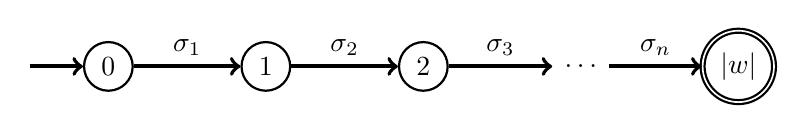
\begin{tikzpicture}[baseline={(current bounding box.center)}]
% \draw[help lines] (0,0) grid (7,2);
\node (s0) [circle,draw=black,thick] at (0,0) {$0$};
\node (s1) [circle,draw=black,thick] at (2,0) {$1$};
\node (s2) [circle,draw=black,thick] at (4,0) {$2$};
\node (sdots) [circle,draw=white,thick] at (6,0) {$\ldots$};
\node (sn) [circle,draw=black,thick,double] at (8,0) {$|w|$};
%
\path[->,line width=0.5mm](-1,0) edge (s0);
\path[->,line width=0.5mm](s0) edge node[above] {$\sigma_1$} (s1);
\path[->,line width=0.5mm](s1) edge node[above] {$\sigma_2$} (s2);
\path[->,line width=0.5mm](s2) edge node[above] {$\sigma_3$} (sdots);
\path[->,line width=0.5mm](sdots) edge node[above] {$\sigma_n$} (sn);
\end{tikzpicture}
\bigskip

\codebox{
\emph{Eingabe:} NFA $\Smach{M}=\tuple{Q,\Sigma,\delta,Q_0,F}$ und Wort $w$\\
\emph{Ausgabe:} Ist $w\in\Slang{L}(\Smach{M})$?
\begin{enumerate}[(1)]
	\item Konstruiere $\Smach{M}_w$
	\item Berechne Produktautomat $\Smach{M}\otimes \Smach{M}_w$
	\item Entscheide ob $\Slang(\Smach{M}\otimes \Smach{M}_w)\neq\emptyset$
\end{enumerate}
}

\end{frame}

\begin{frame}\frametitle{Das Wortproblem für NFAs}

Was tun, wenn ein NFA gegeben ist?
\begin{enumerate}[{Variante} 1:]
\item \alert{NFA in DFA umwandeln (Potenzmengenkonstruktion),\\ Wortproblem für DFA lösen}\\
	Exponentieller Algorithmus: Potenzmengen-DFA ist exponentiell groß
\item \alert{NFA direkt mit Zustandsmengen simulieren\\ (vergleichbar "`on-the-fly Version von Variante 1"')}\\
	Polynomieller Algorithmus: Zustandsmengen sind von linearer Größe; Berechnung der Nachfolgemenge als
	Vereinigung linear vieler $\delta$-Ergebnismengen
\item \alert{Konstruiere einen DFA $\Smach{M}_w$ mit $\Slang{L}(\Smach{M}_w)=\{w\}$ und prüfe ob
$\Slang{L}(\Smach{M})\cap \Slang{L}(\Smach{M}_w) \neq\emptyset$}\\
	Polynomieller Algorithmus: $\Smach{M}_w$ ist linear in $|w|$; Schnittmengen-DFA ist quadratisch groß;
	Leerheitstest ist polynomiell in dieser Größe
\end{enumerate}

\end{frame}

\begin{frame}[t]\frametitle{Wortproblem für NFAs -- Komplexität}

\begin{enumerate}[{Variante} 1:]
\item \alert{NFA in DFA umwandeln (Potenzmengenkonstruktion),\\ Wortproblem für DFA lösen}
\item \alert{NFA direkt mit Zustandsmengen simulieren\\ (vergleichbar "`on-the-fly Version von Variante 1"')}
\item \alert{Konstruiere einen DFA $\Smach{M}_w$ mit $\Slang{L}(\Smach{M}_w)=\{w\}$ und prüfe ob
$\Slang{L}(\Smach{M})\cap \Slang{L}(\Smach{M}_w) \neq\emptyset$}
\end{enumerate}

Mit Variante 2 und 3 erhalten wir:\medskip

\theobox{\emph{Satz:} Das Wortproblem für NFAs kann in polynomieller Zeit entschieden werden.}

\end{frame}

\begin{frame}\frametitle{Weitere Probleme für Automaten}

% Wichtig ist auch der Vergleich zweier durch Automaten gegebener Sprachen:

\defbox{
Das \redalert{Endlichkeitsproblem} für FAs über Alphabet $\Sigma$ besteht darin, die folgende Funktion zu berechnen:\\[1ex]
\emph{Eingabe:} ein FA $\Smach{M}$\\
\emph{Ausgabe:} "`ja"' wenn $\Slang{L}(\Smach{M})$ endlich ist; andernfalls "`nein"'
}\pause

Idee wie Pumping-Lemma: unendliche Sprachen erfordern Zyklus\\
$\leadsto$ suche nach Zyklen, die auf einem Pfad von einem Start- zu einem Endzustand liegen (polynomiell)\pause

\defbox{
Das \redalert{Universalitätsproblem} für FAs über Alphabet $\Sigma$ besteht darin, die folgende Funktion zu berechnen:\\[1ex]
\emph{Eingabe:} ein FA $\Smach{M}$\\
\emph{Ausgabe:} "`ja"' wenn $\Slang{L}(\Smach{M})=\Sigma^*$; andernfalls "`nein"'
}\pause

Komplement des Leerheitsproblems: $\Slang{L}(\Smach{M})=\Sigma^*$ wenn $\Slang{L}(\overline{\Smach{M}})=\emptyset$\\
$\leadsto$ Komplexität abhängig von FA-Komplementierung


\end{frame}


\begin{frame}\frametitle{Zusammenfassung und Ausblick}

Es gibt viele \redalert{nichtreguläre Sprachen}, was man mit verschiedenen Methoden beweisen kann (Myhill-Nerode, Abschlusseigenschaften, Pumping)
\bigskip

\redalert{$\{\Sterm{a}^n\Sterm{b}^n\mid  n\geq 0\}$ ist nicht regulär}, da FAs nicht zählen können
\bigskip

Algorithmische Probleme zu Automaten sind \redalert{Leerheit, Inklusion, Äquivalenz, Universalität, Endlichkeit} und das \redalert{Wortproblem}
\bigskip

Für DFAs können sie in polynomieller Zeit gelöst werden, für NFAs dagegen zum Teil nur in exponentieller

\anybox{yellow}{
Offene Fragen:
\begin{itemize}
\item Wir haben schon so viel über reguläre Sprachen gelernt -- könnten wir das bitte noch einmal alles zusammenfassen?
\item Und was ist mit kontextfreien Sprachen?
\end{itemize}
}

\end{frame}


\end{document}
